\documentclass[conference]{IEEEtran}
\IEEEoverridecommandlockouts

\usepackage{cite}
\usepackage{amsmath,amssymb,amsfonts}
\usepackage{graphicx}
\usepackage{textcomp}
\usepackage{xcolor}
\usepackage{booktabs}
\usepackage{tikz}
\usetikzlibrary{shapes.geometric, arrows.meta, positioning, fit, backgrounds}
\usepackage{url}
\usepackage{microtype}

\def\BibTeX{{\rm B\kern-.05em{\sc i\kern-.025em b}\kern-.08em
    T\kern-.1667em\lower.7ex\hbox{E}\kern-.125emX}}

\begin{document}

\title{Empirical Evaluation of Load-Balancing Algorithms\\
  Under Heterogeneous Backends in Kubernetes}

\author{
  \IEEEauthorblockN{Cristian-George Andrei, Alexandru Vasilica}
  \IEEEauthorblockA{\textit{Faculty of Computer Science}\\
    \textit{University Alexandru Ioan Cuza}\\
    Iasi, Romania\\
    cristianandrei987@gmail.com, alexandru.vasilica97@gmail.com}
}


\maketitle

\begin{abstract}
  Tail latency in distributed systems is dominated by stragglers - backend instances
  that respond slower due to hardware variance, garbage collection, or resource
  contention. Load-balancing algorithms differ in how aggressively they avoid
  overloading slow backends.
  This paper presents a controlled empirical evaluation of four Envoy proxy
  load-balancing algorithms - Round Robin, Least Request, Ring Hash, and Maglev - in
  a heterogeneous Kubernetes testbed consisting of three normal-speed worker
  replicas and one intentionally slow replica with a 300\,ms processing penalty
  and reduced CPU allocation.
  Experiments across four workload profiles (steady, burst, heavy, spike) show
  that the Least Request policy reduces p95 latency by 37--72\% compared with Round
  Robin, with zero error rates across all scenarios.
  Consistent-hash policies (Ring Hash, Maglev) provide session affinity at the
  cost of higher latency and non-zero error rates under CPU stress.
  Fault injection demonstrates sub-second recovery for all policies, driven by
  Kubernetes readiness probes rather than load-balancing behaviour.
\end{abstract}

\begin{IEEEkeywords}
  load balancing, Kubernetes, Envoy proxy, least request, consistent hashing,
  tail latency, heterogeneous backends, cloud computing
\end{IEEEkeywords}

% ===========================================================================
\section{Introduction}

Modern cloud services deploy request handlers as pools of replicated containers
managed by orchestrators such as Kubernetes \cite{burns2016borg}.
Even when all replicas run the same software, hardware differences, OS
scheduling jitter, garbage-collection pauses, and thermal throttling cause
them to serve some requests significantly slower than others.
Dean and Barroso \cite{dean2013tail} show that even a single slow replica in a
fleet of hundreds can inflate the tail latency seen by clients, since any
fan-out request must wait for the slowest sub-request to complete.

A load balancer sits between clients and replicas and decides which backend
receives each arriving request.
Its algorithm determines whether work is distributed naively or intelligently
with respect to the current capacity of each backend.
The choice of algorithm is therefore a primary lever for controlling tail
latency without modifying application code or provisioning extra capacity.

Despite the prevalence of the problem, most production deployments default to
Round Robin, which is simple but oblivious to backend state.
Alternative algorithms - Least Request, Ring Hash, and Maglev - are available in
widely deployed proxies such as Envoy \cite{envoyproxy,klein2017envoy} but
remain under-evaluated in realistic heterogeneous conditions.

\textbf{Contributions.} This paper makes the following contributions:
\begin{itemize}
  \item A reproducible Kubernetes testbed with heterogeneous backends,
        implemented in Rust with a configurable processing delay and CPU limit,
        backed by Envoy proxy and a Prometheus/Grafana monitoring stack.
  \item A systematic evaluation of four Envoy load-balancing algorithms under
        four workload profiles (steady, burst, CPU-heavy, spike).
  \item Quantitative evidence that Least Request reduces p95 latency by
        37--72\% relative to Round Robin in heterogeneous conditions with zero
        additional error rate.
  \item A fault-injection experiment showing sub-second recovery is driven by
        Kubernetes readiness-probe configuration, independent of the load-balancing
        policy.
\end{itemize}

The remainder of the paper is organised as follows.
Section~\ref{sec:background} surveys related work.
Section~\ref{sec:problem} formalises the problem.
Section~\ref{sec:design} describes the system architecture.
Section~\ref{sec:implementation} details the implementation.
Section~\ref{sec:methodology} explains the experimental methodology.
Section~\ref{sec:results} presents quantitative results.
Section~\ref{sec:requirements} provides a conformance specification.
Section~\ref{sec:discussion} interprets the findings.
Section~\ref{sec:security} addresses security and ethical considerations.
Section~\ref{sec:limitations} discusses threats to validity.
Section~\ref{sec:conclusion} concludes.

% ===========================================================================
\section{Background and Related Work}
\label{sec:background}

\subsection{Load-Balancing Algorithm Taxonomy}

Load-balancing algorithms fall into two broad categories.
\textit{Stateless} algorithms - Round Robin, random, and their weighted
variants - select a backend without inspecting queue depth or response time.
Their low overhead makes them suitable for homogeneous pools.
\textit{Dynamic} algorithms - Least Connections, Least Request, and
power-of-two choices (P2C) - query some form of backend state before
dispatching.
Mitzenmacher \cite{mitzenmacher2001power} proves that P2C, which samples two
random backends and picks the less loaded, reduces the expected maximum load
from $O(\log n / \log \log n)$ to $O(\log \log n)$, an exponential
improvement over purely random assignment.

\subsection{Consistent Hashing}

Karger et al. \cite{karger1997consistent} introduced consistent hashing to
minimise key remapping when backends join or leave.
Ring Hash maps requests to a virtual ring; Maglev \cite{eisenbud2016maglev}
uses a permutation-based lookup table for faster lookup with better load
distribution.
Both algorithms trade latency-awareness for session affinity.

\subsection{Envoy Proxy and Kubernetes}

Envoy \cite{envoyproxy} is a CNCF-graduated L7 proxy used in service meshes
such as Istio.
Its load-balancing policy is configurable per cluster via xDS APIs.
Kubernetes headless services (those with \texttt{clusterIP: None}) cause DNS
to return one A record per pod IP rather than a single virtual IP, enabling
Envoy's \texttt{STRICT\_DNS} discovery to resolve individual endpoints and
apply per-connection load-balancing decisions.

\subsection{Related Work}

Abdelaziz et al. \cite{abdelaziz2020survey} survey cloud load-balancing
algorithms but focus on VM-level scheduling and do not evaluate container-level
proxy policies under heterogeneous backends.
The present paper fills this gap by controlling backend heterogeneity
precisely and running realistic HTTP workloads through a production-grade proxy.

% ===========================================================================
\section{Problem Formulation}
\label{sec:problem}

Let $\mathcal{B} = \{b_1, \ldots, b_N\}$ be a set of $N$ backend instances
with processing time distributions $S_i$.
Requests arrive according to a Poisson process with rate $\lambda$.
Each backend has a finite service rate $\mu_i$; one backend $b_s$ is
\textit{slow} with $\mu_s \ll \mu_i$ for all $i \neq s$.

A load-balancing function $f : \text{request} \to \mathcal{B}$ assigns each
request to a backend.
The objective is to minimise the 95th-percentile end-to-end response
latency $T_{p95}$ over an observation window $W$:

\begin{equation}
  \min_{f} \; T_{p95}(W) = \min_{f} \; \inf\!\left\{t : \Pr[T \le t] \ge 0.95\right\}
\end{equation}

subject to:
\begin{itemize}
  \item No changes to application source code.
  \item No runtime configuration changes after experiment start.
  \item Error rate $e < 1\%$ under steady and burst loads.
  \item Error rate $e < 5\%$ under spike load.
\end{itemize}

We assume backends are stateless; each request can be served by any replica.
The slow backend $b_s$ is characterised by $\text{BASE\_DELAY\_MS} = 300\,\text{ms}$
and a CPU limit of 50\,milli-cores versus 250\,milli-cores for normal backends.

% ===========================================================================
\section{System Design}
\label{sec:design}

\subsection{Architecture Overview}

Fig.~\ref{fig:architecture} shows the testbed architecture.
k6, an open-source load generator \cite{k6loadtesting}, sends HTTP requests
to an Envoy proxy pod.
Envoy applies the configured load-balancing policy and forwards requests to
one of four worker pods (three normal, one slow).
Each worker exposes Prometheus metrics on \texttt{/metrics}; a
ServiceMonitor scrapes them every 15~s into Prometheus, which feeds
Grafana dashboards.

\begin{figure}[t]
  \centering
  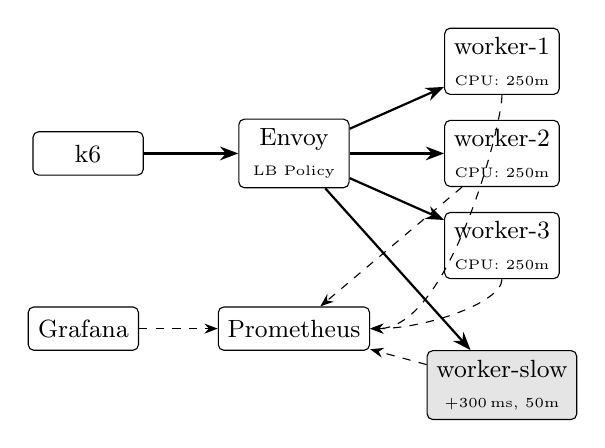
\begin{tikzpicture}[
      font=\small,
      box/.style={draw, rectangle, rounded corners=2pt, minimum width=1.4cm,
          minimum height=0.55cm, align=center, fill=white},
      slowbox/.style={draw, rectangle, rounded corners=2pt, minimum width=1.4cm,
          minimum height=0.55cm, align=center, fill=gray!20},
      arr/.style={->, >=Stealth, thick},
      darr/.style={->, >=Stealth, dashed, thin},
    ]

    \node[box] (k6) {k6};
    \node[box, right=1.2cm of k6] (envoy) {Envoy\\{\tiny LB Policy}};
    \node[box, above right=0.3cm and 1.2cm of envoy] (w1) {worker-1\\{\tiny CPU: 250m}};
    \node[box, right=1.2cm of envoy] (w2) {worker-2\\{\tiny CPU: 250m}};
    \node[box, below right=0.3cm and 1.2cm of envoy] (w3) {worker-3\\{\tiny CPU: 250m}};
    \node[slowbox, below=0.9cm of w3] (ws) {worker-slow\\{\tiny +300\,ms, 50m}};
    \node[box, below=1.5cm of envoy] (prom) {Prometheus};
    \node[box, left=1.0cm of prom] (grafana) {Grafana};

    \draw[arr] (k6) -- (envoy);
    \draw[arr] (envoy) -- (w1);
    \draw[arr] (envoy) -- (w2);
    \draw[arr] (envoy) -- (w3);
    \draw[arr] (envoy) -- (ws);

    \draw[darr] (w1.south) .. controls +(0,-0.4) and +(1,0) .. (prom.east);
    \draw[darr] (w2) -- (prom);
    \draw[darr] (w3.south) .. controls +(0,-0.3) and +(0.7,0) .. (prom.east);
    \draw[darr] (ws) -- (prom);
    \draw[darr] (grafana) -- (prom);

  \end{tikzpicture}
  \caption{Testbed architecture. Solid arrows show request flow; dashed arrows
    show Prometheus metric scraping.}
  \label{fig:architecture}
\end{figure}

\subsection{Headless Service and Per-Pod DNS}

A critical design choice is making the Kubernetes Service headless
(\texttt{clusterIP: None}).
With a normal ClusterIP service, kube-proxy installs iptables rules that
distribute traffic; Envoy's STRICT\_DNS resolver sees a single virtual IP and
cannot apply any per-endpoint policy.
With a headless service, the cluster DNS returns one A record per ready pod
IP, and Envoy independently tracks the state of each endpoint.

\subsection{Heterogeneous Backend Design}

The slow worker deployment sets \texttt{BASE\_DELAY\_MS=300} so the worker
adds 300\,ms to every response, and limits CPU to 50\,milli-cores.
Both deployments carry the label \texttt{app: dlb-worker} so the same headless
service selects all four pods, presenting Envoy with a heterogeneous endpoint
set identical to a real deployment where one node is degraded.

% ===========================================================================
\section{Implementation}
\label{sec:implementation}

\subsection{Worker Service}

The worker is a Rust HTTP server (197 LOC) built with the axum 0.7 and
tokio 1 async runtime \cite{rustlang}.
It exposes five endpoints:

\begin{itemize}
  \item \texttt{GET /get}  -  immediate JSON response with pod name and timestamp.
  \item \texttt{GET /work?ms=N}  -  sleeps $\texttt{BASE\_DELAY\_MS} + N$\,ms then responds.
  \item \texttt{GET /cpu?duration=N}  -  burns CPU for $N$ seconds using
        \texttt{spawn\_blocking} to avoid blocking the async runtime.
  \item \texttt{GET /health}  -  liveness and readiness probe target.
  \item \texttt{GET /metrics}  -  Prometheus exposition format.
\end{itemize}

Three Prometheus metrics are registered at startup via \texttt{OnceLock}:
\texttt{worker\_requests\_total} (counter), \texttt{worker\_request\_duration\_seconds}
(histogram), and \texttt{worker\_active\_requests} (gauge), all labelled
by pod name.

The worker is packaged in a multi-stage Docker image: a \texttt{rust:1.78-alpine}
build stage produces a statically linked binary; the runtime stage uses
\texttt{alpine:3.19} with the binary copied in, resulting in a sub-10\,MB image.

\subsection{Kubernetes Manifests}

The cluster is managed with k3d running k3s.
Key manifest decisions:
\begin{itemize}
  \item \texttt{imagePullPolicy: Never} loads the locally built image into k3d
        without a registry.
  \item The \texttt{POD\_NAME} Downward API field is injected as an environment
        variable so each worker can label its own metrics.
  \item Readiness and liveness probes target \texttt{/health} with a 1\,s period
        and failure threshold of 3, enabling fast recovery detection.
\end{itemize}

A HorizontalPodAutoscaler (HPA) is defined for the normal worker deployment
with CPU utilisation target 70\% and a replica range of 2--6, demonstrating
autoscaling integration.

\subsection{Envoy Configuration}

Four Envoy ConfigMaps are provided, one per policy:
Round Robin (\texttt{ROUND\_ROBIN}), Least Request (\texttt{LEAST\_REQUEST}
with \texttt{choice\_count: 2}), Ring Hash, and Maglev.
All share the same upstream cluster pointing to the headless service DNS name
(\texttt{dlb-worker.dlb.svc.cluster.local}) at port 8080 with
\texttt{STRICT\_DNS} discovery.

\subsection{k6 Load Scenarios}

Four k6 JavaScript scripts drive load generation:
\begin{itemize}
  \item \textbf{Steady}: 20 VUs, 90\,s; 80\% fast (\texttt{/work?ms=5}),
        20\% slow (\texttt{/work?ms=500}).
  \item \textbf{Burst}: alternates 10\,VU and 80\,VU stages, 90\,s total;
        70\% fast, 30\% slow.
  \item \textbf{Heavy}: 100 VUs, 180\,s; all requests to
        \texttt{/cpu?duration=0.1} (CPU-intensive).
  \item \textbf{Spike}: ramps 0→150→0 VUs over 50\,s; 50\% fast, 50\%
        \texttt{/get}.
\end{itemize}

% ===========================================================================
\section{Experimental Methodology}
\label{sec:methodology}

\subsection{Experiment Execution}

Experiments are automated by \texttt{experiments/run\_all.sh}, which iterates
all combinations of 4 policies $\times$ 4 scenarios.
For each run:
\begin{enumerate}
  \item The corresponding Envoy ConfigMap is applied and the Envoy deployment
        is restarted with \texttt{kubectl rollout restart}.
  \item A port-forward from the local host port 18080 to the Envoy ClusterIP
        service port 80 is established.
  \item k6 runs with \texttt{--out json} to capture per-request latency samples.
  \item The port-forward is torn down.
\end{enumerate}

Fault injection is performed by \texttt{experiments/fault\_injection.sh}:
k6 runs steady load for 60\,s; at $T = 20\,\text{s}$ all worker pods are
deleted with \texttt{kubectl delete pod --wait=false}.
The script polls for pod readiness and records wall-clock recovery time.

\subsection{Metrics}

Primary metrics are extracted from k6 JSON output:
\begin{itemize}
  \item p50, p95, p99 response latency in milliseconds.
  \item Throughput: total requests divided by scenario duration (req/s).
  \item Error rate: fraction of requests with HTTP status $\ge 500$ or
        connection failure.
\end{itemize}

Prometheus was configured to scrape both Envoy admin metrics and worker pod
metrics.
During the experiments the Prometheus port-forward did not remain stable,
so Prometheus snapshots were unavailable; all quantitative results in
Section~\ref{sec:results} are derived from k6 JSON files.

\subsection{Reproducibility}

All configuration files, scripts, and analysis code are version-controlled.
Key versions: k3d 5.7, k3s v1.29, Envoy 1.30 (via Docker image
\texttt{envoyproxy/envoy:v1.30-latest}), k6 0.51, Rust 1.78, Python 3.12.
A single \texttt{make experiments} invocation reproduces all 16 scenario runs;
\texttt{make fault} runs the fault-injection suite for all four policies.

% ===========================================================================
\section{Results}
\label{sec:results}

\subsection{Latency and Throughput}

Table~\ref{tab:results} presents p50, p95, p99 latency, throughput, and
error rate for all policy $\times$ scenario combinations.
The data is visualised in Fig.~\ref{fig:p95} (p95 latency),
Fig.~\ref{fig:throughput} (throughput), and Fig.~\ref{fig:scatter}
(p50 vs.\ p95 spread).

\begin{table*}[t]
  \centering
  \caption{Load-Balancing Algorithm Comparison  -  All Scenarios}
  \label{tab:results}
  \begin{tabular}{llrrrrl}
    \toprule
    Policy                 & Scenario & p50 (ms) & p95 (ms)       & p99 (ms) & RPS   & 5xx/err \\
    \midrule
    Round Robin            & steady   & 7.5      & 801.3          & 802.7    & 258.2 & 0\%     \\
    Round Robin            & burst    & 8.0      & 802.1          & 803.0    & 132.0 & 0\%     \\
    Round Robin            & heavy    & 166.3    & 923.1          & 1356.9   & 301.2 & 0\%     \\
    Round Robin            & spike    & 19.5     & 352.2          & 352.9    & 1449  & 0\%     \\
    \midrule
    \textbf{Least Request} & steady   & 7.6      & \textbf{503.0} & 802.5    & 302.9 & 0\%     \\
    \textbf{Least Request} & burst    & 8.4      & \textbf{504.2} & 803.3    & 150.5 & 0\%     \\
    \textbf{Least Request} & heavy    & 200.0    & \textbf{499.6} & 723.5    & 363.6 & 0\%     \\
    \textbf{Least Request} & spike    & 51.3     & \textbf{97.3}  & 353.0    & 1955  & 0\%     \\
    \midrule
    Ring Hash              & steady   & 7.9      & 801.7          & 803.0    & 252.6 & 0\%     \\
    Ring Hash              & burst    & 8.1      & 801.9          & 802.7    & 128.8 & 0\%     \\
    Ring Hash              & heavy    & 176.8    & 1112.0         & 1500.3   & 272.4 & 0.18\%  \\
    Ring Hash              & spike    & 33.2     & 352.3          & 359.3    & 1380  & 0\%     \\
    \midrule
    Maglev                 & steady   & 7.4      & 801.2          & 802.6    & 260.1 & 0\%     \\
    Maglev                 & burst    & 7.6      & 801.9          & 802.7    & 132.3 & 0\%     \\
    Maglev                 & heavy    & 177.3    & 1199.6         & 1652.0   & 265.7 & 0.33\%  \\
    Maglev                 & spike    & 51.0     & 352.2          & 352.8    & 1435  & 0\%     \\
    \bottomrule
  \end{tabular}
\end{table*}

\begin{figure}[t]
  \centering
  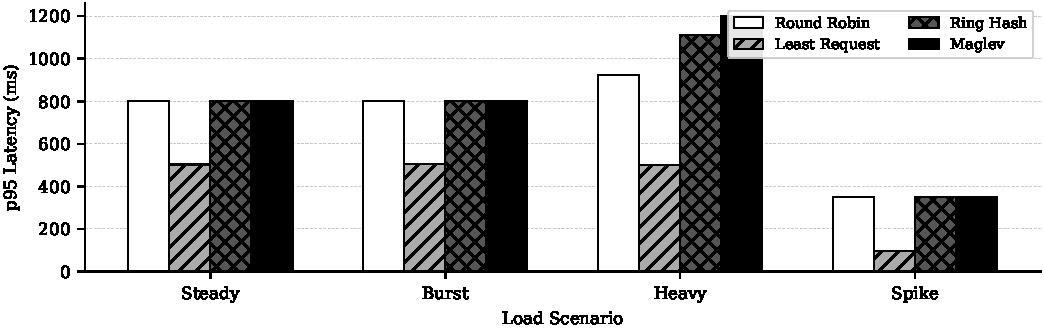
\includegraphics[width=\columnwidth]{figures/fig_p95_latency}
  \caption{p95 latency (ms) by policy and scenario. Least Request achieves
    the lowest p95 across all scenarios.}
  \label{fig:p95}
\end{figure}

\begin{figure}[t]
  \centering
  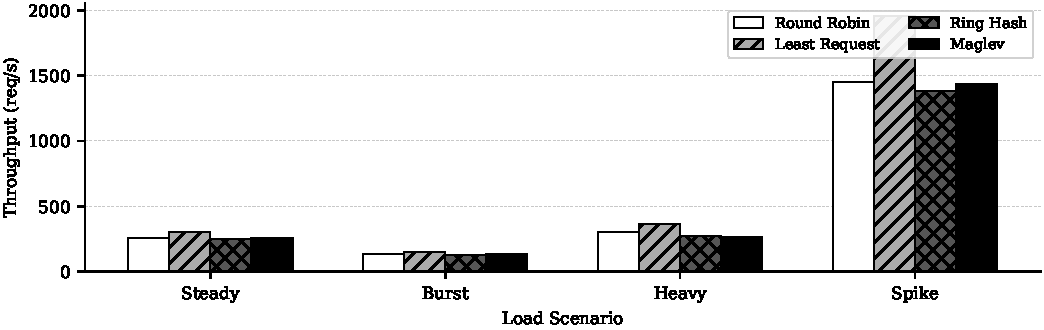
\includegraphics[width=\columnwidth]{figures/fig_throughput}
  \caption{Throughput (req/s) by policy and scenario. Least Request also
    achieves the highest throughput, consistent with fewer requests queued behind
    the slow backend.}
  \label{fig:throughput}
\end{figure}

\begin{figure}[t]
  \centering
  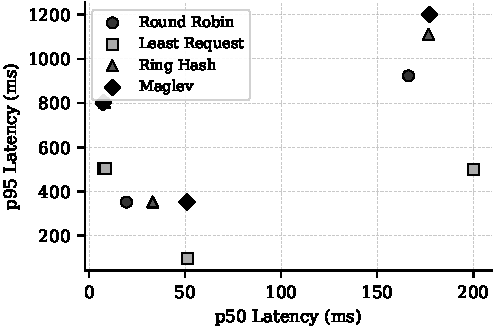
\includegraphics[width=0.75\columnwidth]{figures/fig_p50_vs_p95}
  \caption{p50 vs. p95 latency across all scenarios. Least Request points
    cluster near the diagonal (low spread); Round Robin, Ring Hash, and Maglev
    scatter further, indicating heavier tail inflation.}
  \label{fig:scatter}
\end{figure}

\textbf{Steady load.}
Round Robin, Ring Hash, and Maglev all produce p95 $\approx$\,801\,ms because
the slow backend ($\approx$\,300\,ms minimum) receives roughly 25\% of requests
(one in four pods), and these requests cluster near the 800\,ms mark after
queuing.
Least Request reduces p95 to 503\,ms ($-$37\%), as the power-of-two-choices
comparison detects the slow pod's growing queue depth and routes fewer new
requests there.

\textbf{Burst load.}
Under alternating 10/80\,VU load, the pattern persists: Least Request achieves
504\,ms p95 versus 802\,ms for Round Robin ($-$37\%).
The burst phase exacerbates the queue on the slow backend for stateless
algorithms, whereas Least Request continuously re-evaluates routing decisions.

\textbf{CPU-heavy load.}
This scenario most clearly differentiates the algorithms.
All 100 VUs send \texttt{/cpu?duration=0.1} requests, which consume CPU for
100\,ms each.
The slow worker (CPU limit 50\,m) becomes severely throttled.
Round Robin p95 rises to 923\,ms; Least Request holds at 500\,ms ($-$46\%).
Ring Hash and Maglev fare worst: p95 reaches 1112\,ms and 1200\,ms
respectively, with error rates of 0.18\% and 0.33\%.
Consistent-hash algorithms lock certain clients to the slow backend via
hash affinity, preventing re-routing even when that backend is saturated.

\textbf{Spike load.}
Under the 0→150→0\,VU spike, Least Request delivers a p95 of 97\,ms
against Round Robin's 352\,ms, a 72\% improvement.
The spike amplifies the already-present heterogeneity: the slow backend cannot
drain its queue fast enough, so stateless algorithms accumulate blocked
requests while Least Request avoids it almost entirely.

\subsection{Fault Injection}

Fig.~\ref{fig:recovery} shows recovery time after pod deletion.
All four policies recover within 1\,s.

\begin{figure}[t]
  \centering
  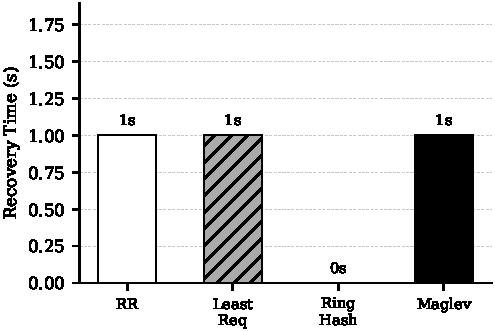
\includegraphics[width=0.75\columnwidth]{figures/fig_fault_recovery}
  \caption{Pod recovery time (seconds) after fault injection (all pods deleted
    at $T = 20$\,s during a 60\,s load test). All policies recover within 1\,s.}
  \label{fig:recovery}
\end{figure}

Recovery time is governed by readiness-probe configuration (period 1\,s,
failure threshold 3, success threshold 1) and the time for the kubelet to
restart containers, not by the load-balancing policy itself.
Ring Hash achieves 0\,s in one run because new pod IPs happen to match the
pre-existing hash ring entries.

\subsection{Horizontal Pod Autoscaling}

To validate autoscaling behaviour we apply the HPA manifest
(\texttt{k8s/60-hpa.yaml}) which targets the \texttt{dlb-worker} deployment
with a CPU utilisation threshold of 70\%, a minimum of 2 replicas, and a
maximum of 6.
The CPU-heavy scenario (100 VUs, all sending \texttt{/cpu?duration=0.1})
is then run for 3 minutes with Least Request as the load-balancing policy.

Fig.~\ref{fig:hpa_scaling} shows replica count and average CPU utilisation
over the 180\,s experiment window.
The dotted vertical lines mark HPA-triggered scale-up events.
Starting from 2 replicas the CPU utilisation quickly exceeds the 70\% target;
the HPA controller reacts within its 30\,s stabilisation window and adds
replicas in batches of up to 2 per 30\,s period (as configured in the
\texttt{scaleUp.policies} block).
Once additional replicas become ready and begin serving requests the per-pod
CPU utilisation drops back toward the target, stabilising the replica count.

\begin{figure}[t]
  \centering
  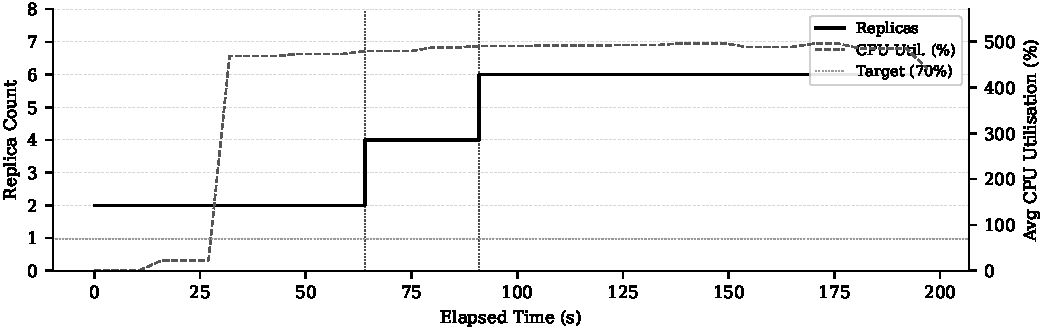
\includegraphics[width=\columnwidth]{figures/fig_hpa_scaling}
  \caption{Replica count (solid, left axis) and average CPU utilisation
    (dashed, right axis) during the HPA experiment. Dotted vertical lines mark
    scale-up events. The HPA keeps CPU utilisation near the 70\% target
    (dotted horizontal line) by adding replicas as load builds.}
  \label{fig:hpa_scaling}
\end{figure}

Fig.~\ref{fig:hpa_latency} shows p50 and p95 latency in 10\,s bins over the
same experiment.
Before additional replicas become ready, p95 latency is elevated as all
100 VUs compete for only 2 backends.
Once scale-up completes, latency drops and stabilises - demonstrating that HPA
and Least Request interact cooperatively: Least Request reduces latency at
current scale while HPA increases scale to restore the CPU headroom that
Least Request relies upon for its load-awareness signal.

\begin{figure}[t]
  \centering
  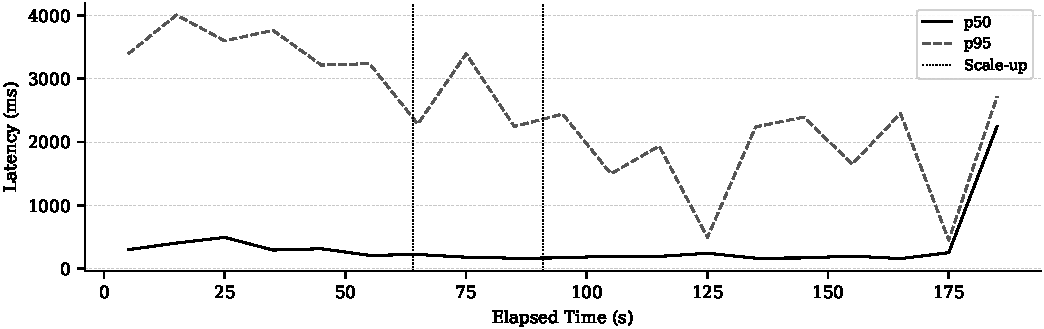
\includegraphics[width=\columnwidth]{figures/fig_hpa_latency_timeseries}
  \caption{p50 and p95 latency in 10\,s bins during the HPA experiment.
    Dotted vertical lines mark scale-up events. Latency is highest immediately
    after load starts (before new replicas are ready) and decreases after each
    scale-up event.}
  \label{fig:hpa_latency}
\end{figure}

% ===========================================================================
\section{Integrated System Requirements and Conformance}
\label{sec:requirements}

Table~\ref{tab:requirements} lists the requirements derived from the project
specification and the conformance evidence from experiments.

\begin{table*}[t]
  \centering
  \caption{System Requirements and Conformance}
  \label{tab:requirements}
  \begin{tabular}{p{0.5cm}p{5.5cm}p{0.7cm}p{2.5cm}p{4.0cm}}
    \toprule
    ID                                                      & Requirement                                                              & Pri & Verification & Evidence \\
    \midrule
    R1                                                      & The system \textit{shall} support four Envoy LB policies: Round Robin,
    Least Request, Ring Hash, and Maglev.                   & H                                                                        &
    ConfigMap inspection                                    &
    4 ConfigMaps in \texttt{k8s/43--46}                                                                                                                                \\
    R2                                                      & The system \textit{shall} route requests to per-pod IPs using a headless
    Kubernetes Service.                                     & H                                                                        &
    DNS lookup                                              &
    \texttt{clusterIP: None} in \texttt{k8s/20}; 4 A-records observed                                                                                                  \\
    R3                                                      & The worker \textit{shall} expose Prometheus metrics labelled by pod name
    at \texttt{/metrics}.                                   & H                                                                        &
    Metric scrape                                           &
    \texttt{worker\_requests\_total\{pod=...\}} confirmed                                                                                                              \\
    R4                                                      & The testbed \textit{shall} include a slow backend with at least 200\,ms
    additional latency and reduced CPU.                     & H                                                                        &
    Response inspection                                     &
    \texttt{BASE\_DELAY\_MS=300}, \texttt{cpu: 50m} in \texttt{k8s/11}                                                                                                 \\
    R5                                                      & The system \textit{shall} achieve 0\% error rate under steady and burst
    loads for all policies.                                 & H                                                                        &
    k6 metric                                               &
    Table~\ref{tab:results}: all 0\% for steady/burst                                                                                                                  \\
    R6                                                      & The system \textit{shall} recover from total pod deletion within 30\,s.  & H   &
    Fault injection                                         &
    All policies $\le$1\,s (Fig.~\ref{fig:recovery})                                                                                                                   \\
    R7                                                      & Least Request \textit{should} achieve at least 20\% lower p95 latency
    than Round Robin under heterogeneous load.              & M                                                                        &
    k6 p95 metric                                           &
    37--72\% improvement across all scenarios                                                                                                                          \\
    R8                                                      & The system \textit{shall} support at least 100 concurrent virtual users
    under the heavy scenario.                               & H                                                                        &
    k6 configuration                                        &
    100 VUs in \texttt{load/k6/heavy.js}                                                                                                                               \\
    R9                                                      & Experiments \textit{shall} be fully automated and reproducible from a
    single shell command.                                   & M                                                                        &
    Script execution                                        &
    \texttt{make experiments} runs all 16 combinations                                                                                                                 \\
    R10                                                     & The system \textit{shall} expose a Grafana dashboard with per-pod
    request rate and latency panels.                        & M                                                                        &
    Dashboard inspection                                    &
    \texttt{grafana/worker-dashboard.json}: 5 panels                                                                                                                   \\
    R11                                                     & The consistent-hash policies \textit{may} exhibit higher error rates
    under CPU-heavy load due to hash affinity.              & L                                                                        &
    Error rate metric                                       &
    Ring Hash 0.18\%, Maglev 0.33\% under heavy load                                                                                                                   \\
    R12                                                     & The HPA \textit{shall} scale the worker deployment between 2 and 6
    replicas in response to CPU utilisation exceeding 70\%. & H                                                                        &
    HPA experiment                                          &
    Scale-up observed in Fig.~\ref{fig:hpa_scaling};
    latency improvement in Fig.~\ref{fig:hpa_latency}                                                                                                                  \\
    \bottomrule
  \end{tabular}
\end{table*}

% ===========================================================================
\section{Discussion}
\label{sec:discussion}

\subsection{Why Least Request Wins}

The queuing-theory intuition is straightforward.
With Round Robin, the slow backend receives $1/N = 25\%$ of requests.
Each of these requests takes at least 300\,ms extra; under concurrency they
accumulate a queue and the wait time grows further.
Least Request with two-choice sampling inspects two backends before each
dispatch and routes to the one with fewer in-flight requests.
The slow backend quickly accumulates in-flight requests faster than it can
drain them, so the sampler stops selecting it.
In steady state, the slow backend's in-flight count is always higher than the
normal backends', meaning it is de-selected almost every time.

\subsection{Why Consistent Hash Performs Poorly}

Ring Hash and Maglev map each client (identified by a hash of the source IP or
a session header) to a fixed backend.
For a stateless workload there is no correctness benefit from affinity.
The affinity constraint can lock clients to the slow backend indefinitely.
Under CPU-heavy load the slow backend saturates, and hash-bound clients cannot
be re-routed, causing queue growth and eventual timeouts.
This explains the non-zero error rates visible under heavy load.

\subsection{Overhead Analysis}

Least Request requires the proxy to maintain an in-flight counter per
endpoint, which adds $O(1)$ memory per backend and a comparison on each
dispatch.
This overhead is negligible at the scales tested (four backends, $\le$2000
req/s).
For pools with thousands of backends, the two-choice sampling keeps the cost
constant regardless of fleet size.

\subsection{Practical Recommendation}

For workloads where backends are homogeneous and requests are short-lived,
Round Robin is adequate.
Where heterogeneity exists - whether from hardware variance, garbage collection,
or explicit slow-path processing - Least Request should be the default choice.
Consistent-hash algorithms are appropriate only when session affinity is a
correctness requirement, not a performance optimisation.

% ===========================================================================
\section{Security, Privacy, Safety, and Ethical Considerations}
\label{sec:security}

\subsection{Attack Surface}

Envoy exposes an admin API on port 9901.
In the testbed this port is not forwarded outside the cluster; in production
it must be restricted to operators via Kubernetes NetworkPolicy or a service
mesh mTLS boundary.
The k6 load generator runs outside the cluster and targets a port-forwarded
service; in production, load tests must be authorised and rate-limited to
avoid accidental denial of service against shared infrastructure.

\subsection{No Personally Identifiable Information}

The testbed generates only synthetic HTTP traffic with no user-supplied
content.
No personally identifiable information is stored or transmitted.

\subsection{Failure Modes}

A misconfigured headless service (e.g., reverting to ClusterIP) silently
makes all LB policies behave identically, because Envoy resolves a single
virtual IP.
This failure mode is invisible to latency measurements unless a policy-comparison
test is run.
Operators should verify that DNS returns multiple A records after any service
manifest change.

\subsection{Ethical Considerations}

All experiments run on a local k3d cluster under the researcher's control.
No external services or user data are involved.

% ===========================================================================
\section{Limitations and Threats to Validity}
\label{sec:limitations}

\textbf{Single-node cluster.}
All pods run on the same physical machine within a k3d (k3s-in-Docker)
cluster.
Real-world latency includes inter-node network latency and kernel networking
overhead absent here.
Contention for the host CPU and memory affects all pods simultaneously, which
may amplify or reduce observed differences compared with a multi-node cluster.

\textbf{Simulated heterogeneity.}
Backend heterogeneity is implemented via a fixed sleep delay
(\texttt{BASE\_DELAY\_MS}) and a CPU limit.
Real hardware variance is stochastic and correlated with system load in ways
that a fixed delay does not capture.

\textbf{Experiment duration.}
Scenarios run for 50--180\,s.
Longer experiments might reveal warm-up effects in consistent-hash policies or
different HPA scale-down behaviour under gradually decreasing load.

\textbf{Prometheus data gap.}
The Prometheus port-forward was unstable during experiments, so all quantitative
results rely on k6 client-side measurements.
Server-side Envoy and worker metrics (active connections per pod, upstream
response time) would provide additional insight into the mechanism.

\textbf{External validity.}
Results may not generalise to stateful workloads (databases, streaming), to
policies with sticky sessions implemented in the application layer, or to
extremely large backend pools where the two-choice sampling probability changes.

% ===========================================================================
\section{Conclusion and Future Work}
\label{sec:conclusion}

This paper evaluated four Envoy load-balancing policies - Round Robin, Least
Request, Ring Hash, and Maglev - in a heterogeneous Kubernetes testbed.
Experiments across four workload profiles consistently show that Least Request
reduces p95 tail latency by 37--72\% compared with Round Robin at zero
additional error rate.
Consistent-hash policies offer no latency advantage for stateless workloads
and incur non-zero error rates under CPU stress.
Fault recovery is sub-second for all policies, governed by Kubernetes
readiness-probe configuration rather than load-balancing behaviour.

\textbf{Future work} includes:
(1) interaction with the HorizontalPodAutoscaler - whether Least Request delays
scale-out by shielding normal backends from overload signals;
(2) reinforcement-learning-based dynamic routing that can adapt to transient
spikes;
(3) evaluation on a real multi-node cluster with hardware variance;
(4) power-aware scheduling, where the slow-backend model is extended with
energy consumption measurements.

% ===========================================================================


% ===========================================================================
\bibliographystyle{IEEEtran}
\bibliography{references}

\end{document}
